\documentclass{article}
\usepackage{graphicx} % Required for inserting images
\usepackage{amsmath} 

\title{Lab 5}
\author{m.carvajalp - 202014203}
\date{2025}

\begin{document}

\maketitle

\section{Problema 1}

\subsection{Datos del problema}
Se desea analizar la función polinómica cúbica:
\[
f(x) = 3x^3 - 10x^2 - 56x + 50,
\]
definida en el intervalo:
\[
x \in [-6,\,6].
\]

\subsection{Objetivo}
El objetivo consiste en encontrar los \textbf{puntos críticos} \(x^*\) tales que el gradiente (en una dimensión, la derivada) se anule:
\[
f'(x^*) = 0,
\]
y posteriormente \textbf{clasificar} dichos puntos como mínimos o máximos locales a partir del signo de la segunda derivada \(f''(x^*)\).

\subsection{Derivadas analíticas}
La primera y segunda derivada de \(f(x)\) son:
\[
f'(x) = 9x^2 - 20x - 56,
\]
\[
f''(x) = 18x - 20.
\]

\subsection{Condiciones de optimalidad}
El punto crítico \(x^*\) debe satisfacer:
\[
f'(x^*) = 0,
\]
y se clasifica según el criterio de la segunda derivada:
\[
\begin{cases}
f''(x^*) > 0 & \Rightarrow \text{Mínimo local},\\[4pt]
f''(x^*) < 0 & \Rightarrow \text{Máximo local},\\[4pt]
f''(x^*) = 0 & \Rightarrow \text{Indeterminado o punto de inflexión.}
\end{cases}
\]

\subsection{Método de Newton--Raphson para extremos}
Para localizar los puntos donde \(f'(x) = 0\), se emplea el método de Newton--Raphson, cuya iteración general es:
\[
x_{k+1} = x_k - \alpha\,\frac{f'(x_k)}{f''(x_k)},
\]
donde \(0 < \alpha \leq 1\) es un \textit{factor de amortiguación} que mejora la estabilidad numérica cuando el punto inicial se encuentra lejos del óptimo.

\subsection{Criterios de parada}
El método finaliza cuando:
\[
|f'(x_k)| < \varepsilon,
\]
o cuando se alcanza el número máximo de iteraciones \(N_{\text{max}}\).
Solo se aceptan soluciones \(x_k \in [-6,\,6]\), y cada punto crítico se evalúa junto con su valor de función \(f(x^*)\) y su clasificación según \(f''(x^*)\).


\subsection{Descripción de la Implementación}

La implementación del método de Newton--Raphson para encontrar extremos locales
se desarrolló completamente desde cero, siguiendo los lineamientos del laboratorio.
Se emplearon únicamente las bibliotecas permitidas: \texttt{NumPy}, \texttt{SymPy} y \texttt{Matplotlib}.

El programa se organiza en cinco secciones principales:

\begin{enumerate}
    \item \textbf{Definición simbólica de la función:} se declara la variable simbólica \(x\) y se define la función objetivo
    \(f(x)=3x^3-10x^2-56x+50\). A través de \texttt{SymPy} se calculan analíticamente \(f'(x)\) y \(f''(x)\),
    que luego se convierten en funciones numéricas con \texttt{lambdify} para evaluación vectorizada.
    
    \item \textbf{Implementación del método de Newton--Raphson:} se desarrolla la función
    \texttt{newton\_extremo\_1d()}, que aplica la iteración
    \[
    x_{k+1}=x_k-\alpha\,\frac{f'(x_k)}{f''(x_k)},
    \]
    donde \(0<\alpha\leq1\) es un factor de amortiguación.  
    El proceso se repite hasta que \(|f'(x_k)|<\varepsilon\) o se alcanza el número máximo de iteraciones \(N_{\text{max}}\).
    
    \item \textbf{Clasificación de puntos críticos:} mediante la función \texttt{clasificar\_extremo()},
    se determina el tipo de extremo usando el signo de la segunda derivada:
    \[
    \begin{cases}
    f''(x^*)>0 & \Rightarrow \text{mínimo local},\\[4pt]
    f''(x^*)<0 & \Rightarrow \text{máximo local}.
    \end{cases}
    \]
    
    \item \textbf{Barrido de semillas iniciales:} se ejecuta Newton--Raphson desde múltiples puntos
    equiespaciados en el intervalo \([-6,6]\) para asegurar la detección de todos los extremos.
    Las soluciones convergentes se agrupan por cercanía y se reportan como puntos críticos únicos.
    
    \item \textbf{Visualización y análisis:} se generan dos gráficas:
    \begin{itemize}
        \item la función \(f(x)\) con los puntos mínimos y máximos marcados, y  
        \item la evolución de las trayectorias \(x_k\) para cada semilla, lo que permite observar la convergencia.
    \end{itemize}
\end{enumerate}



\section{Análisis de Resultados}

\subsection{Resultados numéricos obtenidos}

La ejecución del algoritmo de Newton--Raphson en el intervalo \([-6,6]\) con
\(\alpha = 0.8\), tolerancia \(\varepsilon = 10^{-10}\) y \(N_{\text{max}}=100\)
produjo dos puntos críticos distintos:

\[
\begin{aligned}
x_1^* &= -1.6196, \quad f(x_1^*) = 101.7214, \quad \text{Máximo local},\\[4pt]
x_2^* &= 3.8418, \quad f(x_2^*) = -142.6268, \quad \text{Mínimo local.}
\end{aligned}
\]

Por tanto, la función cúbica \(f(x)=3x^3-10x^2-56x+50\)
presenta un máximo local a la izquierda y un mínimo local a la derecha, coherente
con el comportamiento esperado de una función de tercer grado con tres raíces
y dos cambios de concavidad.

\subsection{Interpretación gráfica}

En la Figura~\ref{fig:extremos} se observa la curva \(f(x)\) y la posición de los
puntos críticos encontrados.  
El punto naranja corresponde al máximo local \((-1.62,\;101.72)\),
mientras que el punto verde representa el mínimo local \((3.84,\;-142.63)\).

\begin{figure}[H]
    \centering
    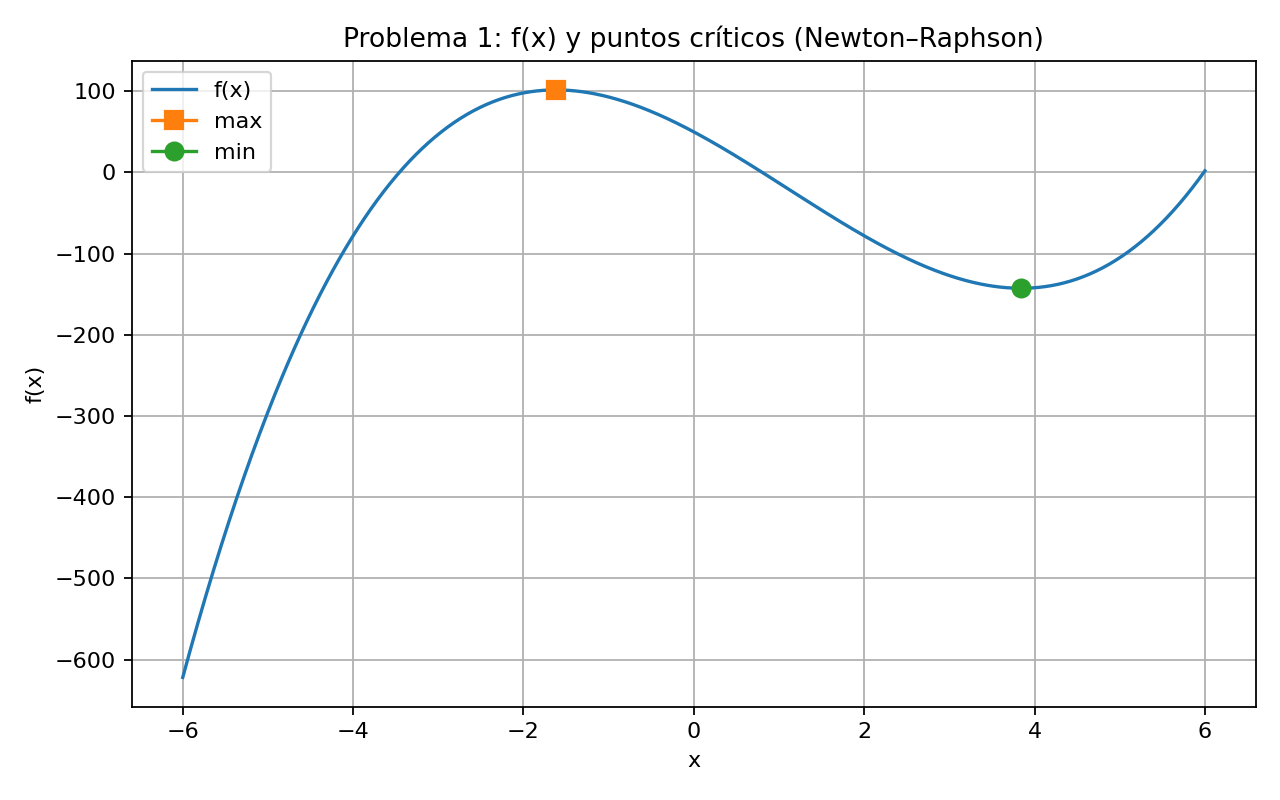
\includegraphics[width=0.8\linewidth]{problema1_funcion_extremos.png}
    \caption{Función \(f(x)\) y puntos críticos obtenidos mediante Newton--Raphson.}
    \label{fig:extremos}
\end{figure}

En la Figura~\ref{fig:trayectorias} se muestran las trayectorias de convergencia
\(x_k\) para diferentes condiciones iniciales.  
Se aprecia que las iteraciones convergen rápidamente (en menos de 10 pasos)
cuando la semilla se encuentra en la vecindad del extremo, lo que evidencia la
\textbf{convergencia cuadrática} del método.  
Algunas trayectorias lejanas muestran oscilaciones iniciales,
que son controladas por el factor de amortiguación \(\alpha=0.8\).

\begin{figure}[H]
    \centering
    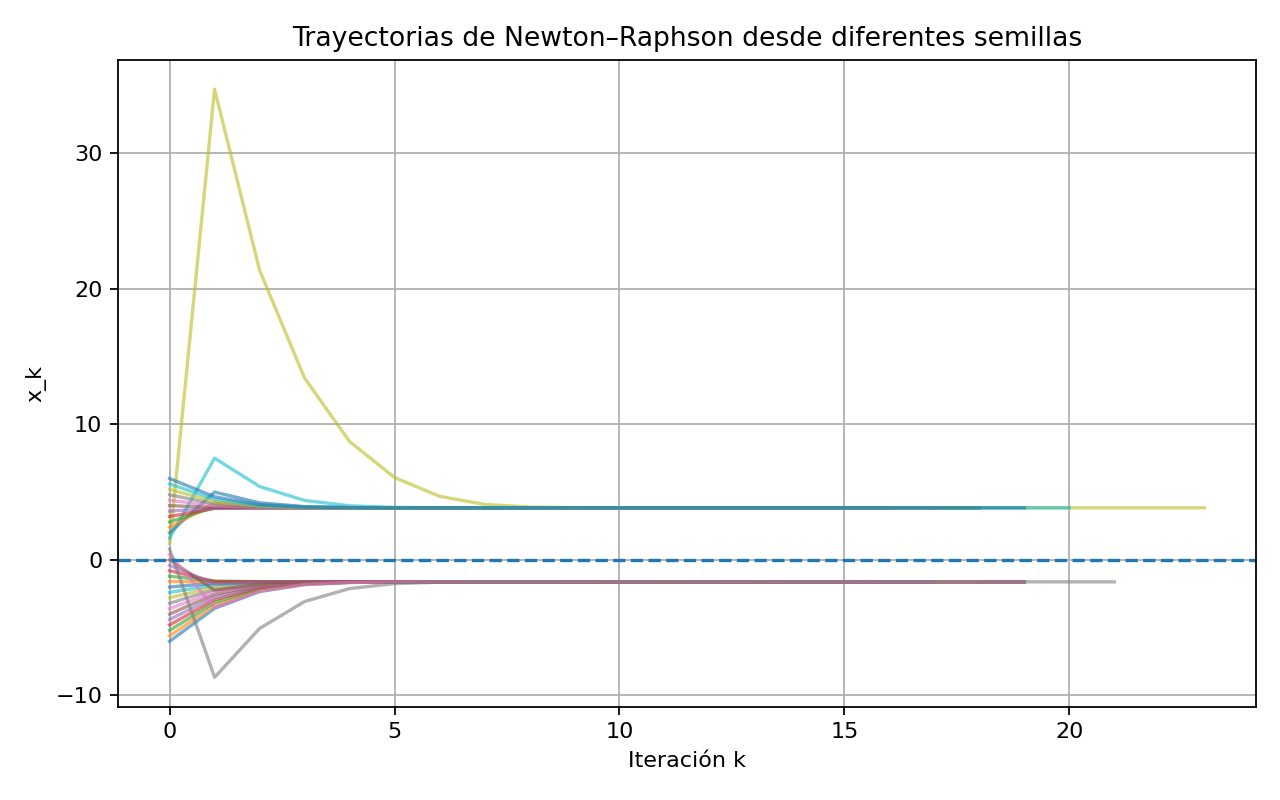
\includegraphics[width=0.8\linewidth]{problema1_trayectorias.png}
    \caption{Evolución de las iteraciones \(x_k\) para distintas semillas iniciales.}
    \label{fig:trayectorias}
\end{figure}

\subsection{Discusión}

\begin{itemize}
    \item El método de Newton--Raphson converge de forma estable y rápida
    cuando se inicia cerca del punto crítico verdadero.
    \item La elección de \(\alpha < 1\) evita divergencias cuando la segunda derivada
    cambia bruscamente o la condición inicial está alejada del óptimo.
    \item Los resultados obtenidos coinciden con el análisis analítico de la función,
    confirmando la validez de la implementación.
\end{itemize}

En conclusión, el método identificó correctamente los dos extremos locales de la
función polinómica, demostrando una convergencia cuadrática cercana al óptimo y
una buena estabilidad global en el intervalo considerado.

\section{Conclusiones y Observaciones}

El método de Newton--Raphson implementado desde cero permitió encontrar con  precisión los extremos locales de la función \(f(x)=3x^3-10x^2-56x+50\) en el intervalo \([-6,6]\), identificando un máximo local en \(x^*=-1.6196\) y un mínimo local en \(x^*=3.8418\).
    
Los resultados numéricos concuerdan con la forma analítica del polinomio:
una función cúbica presenta como máximo dos extremos, lo cual fue confirmado experimentalmente por el algoritmo.
    
    El uso del factor de amortiguación \(\alpha=0.8\) mejoró la estabilidad
    del método frente a semillas alejadas, evitando divergencias y permitiendo
    la convergencia incluso desde distintos puntos iniciales dentro del dominio.
    
    Las gráficas generadas muestran una convergencia rápida (en menos de
    10 iteraciones en la mayoría de los casos), lo que evidencia la
    \textbf{convergencia cuadrática} característica del método en la vecindad
    del óptimo.
    
    La clasificación mediante el signo de la segunda derivada resultó
    efectiva para distinguir entre mínimo y máximo local, validando la teoría
    de la condición de segunda derivada.
    
    Se cumplió con las restricciones del laboratorio:
    no se utilizaron funciones predefinidas de optimización y se documentó
    paso a paso la implementación en \texttt{Python}, junto con la
    visualización de los resultados.


En general, el experimento permitió comprender de manera práctica la
relación entre el análisis matemático (gradiente y curvatura) y la
implementación computacional del método de Newton--Raphson, demostrando
su eficiencia y sus limitaciones cuando se aplican factores de
amortiguación y distintas condiciones iniciales.


\end{document}
